\documentclass[t, notes, xcolor=table]{beamer}

\usepackage{wrapfig}
\usepackage{float}
% For tabs in verbatim
\usepackage{fancyvrb}

% Adjust position of the image
\usepackage[export]{adjustbox}

% set fonts
\usefonttheme{professionalfonts} % using non standard fonts for beamer
\usepackage{txfonts,mathptmx}

% set indend spacing for first and second level indentation
\setlength{\leftmargini}{0.5cm}
\setlength{\leftmarginii}{0.5cm}
\setlength{\leftmarginiii}{0.5cm}

% Set circles for bullets 
\setbeamertemplate{itemize items}[circle]

% colors
\usepackage{xcolor}

% multiple columns
\usepackage{multicol}

% todo lists
\usepackage{pifont}
\usepackage{amssymb}

% increase space between text and frame name
\addtobeamertemplate{frametitle}{}{\vspace{0.5em}}

%Information to be included in the title page:
\title{Introducing the Process of Synthesis}
\author{Nikola Petrovic}
\institute{University of Belgrade, School of Electrical Engineering}
\date{2022}



\begin{document}

\frame{\titlepage}

%%%%%%%%%%%%%%%%%%%%%%%%%%%%%%%%%%%%%%%%%%%%%%%%%%%%%%%%%%%%
\begin{frame}
\frametitle{Module Objective}
In this module we will briefly examine the synthesis process and its results.
\newline

\textbf{Topics:}
\begin{itemize}
\item What is Logic Synthesis?
\item How do we use synthesis?
\item What does synthesis do?
\item What synthesis sometimes can't do well
\item Technology-specific issues
\item Synthesis in our design flow
\item Synthesizable Verilog
\end{itemize}
\end{frame}
\note{
\scriptsize{
Our objective is to be able to briefly describe the synthesis process and its results to team members that are unable to take this course.
\newline

To do that we should know at least somewhat about :
\begin{itemize}
\item How do we use synthesis
\item What does the synthesis tool does
\item Synthesis strengths and weaknesses
\item Technology-specific issues
\item The Verilog language synthesis "subset"
\end{itemize}

}
}


%%%%%%%%%%%%%%%%%%%%%%%%%%%%%%%%%%%%%%%%%%%%%%%%%%%%%%%%%%%%
\begin{frame}
\frametitle{What is Logic Synthesis}
Logic synthesis is a tool that:
\begin{itemize}
\item Infers storage elements (latches, registers)
\item Infers combinational logic feeding storage elements
\item Optimizes generated structure to meed cost factors:
\begin{itemize}
	\item Area / speed / power / routability
\end{itemize}
\end{itemize}
\begin{multicols}{2}
A person new to synthesis might ask:
\begin{itemize}
\item How much of the design?
\item How accurately?
\item How optimally?
\end{itemize}
\vfill
\columnbreak
\begin{figure}
    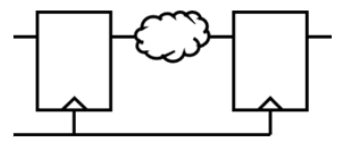
\includegraphics[width=0.35\textwidth]{img/12_logic_synth.png}
\end{figure}
\end{multicols}
\end{frame}
\note{
\scriptsize{
Synthesis automatically transforms our RTL Verilog design into an optimized netlist of predefined cells. Some obvious first questions might be the following:
\begin{itemize}
\item What parts of the design can synthesis handle?
\item Is the result truly functionally equivalent to the RTL?
\item Just how optimal is that result really?
\end{itemize}

}
}

%%%%%%%%%%%%%%%%%%%%%%%%%%%%%%%%%%%%%%%%%%%%%%%%%%%%%%%%%%%%
\begin{frame}
\frametitle{How Do We Use Synthesis?}
\scriptsize{
We provide design source, design constraints, and technology library.

The tool infers logic from that HDL source, maps the inferred logic to the technology library macros, and optimizes the circuit to meet constraints.
}

\begin{figure}
    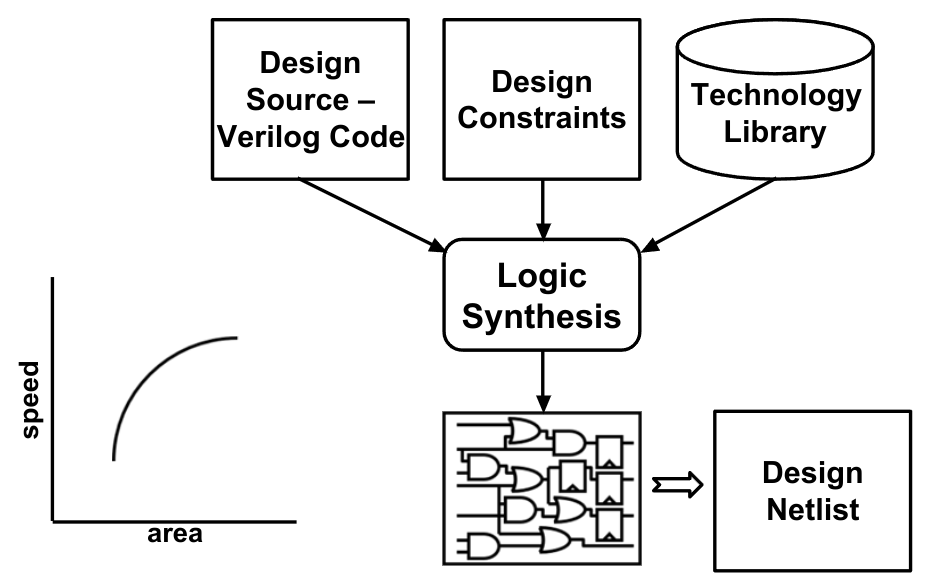
\includegraphics[width=0.95\textwidth]{img/12_how_synth.png}
\end{figure}
\end{frame}
\note{
\scriptsize{
A synthesis tool can read our RTL Verilog code and convert it into a gate level netlist, using gates and cells from a specified target technology library.
\newline

The synthesis tool will try to meed our design constraints for the area and performance, and will produce reports to tell us how successful it was.
\newline

Design constraints include the required clock speed, input drive strength and arrival time with respect to the clock, and output load and required arrival time with respect to the clock. Design constraints can also include power consumption and can sometimes include noise immunity, testability, and factors affecting ease of place and route.
\newline

The synthesis tool trades circuit speed and circuit area. As a general statement, it can produce a small design or a fast design or a compromise between small and fast. Several factors shift the area/speed curve. Among these factors are the target technology and circuit architecture.


}
}

%%%%%%%%%%%%%%%%%%%%%%%%%%%%%%%%%%%%%%%%%%%%%%%%%%%%%%%%%%%%
\begin{frame}
\frametitle{What Foes Synthesis Do?}
\begin{figure}
    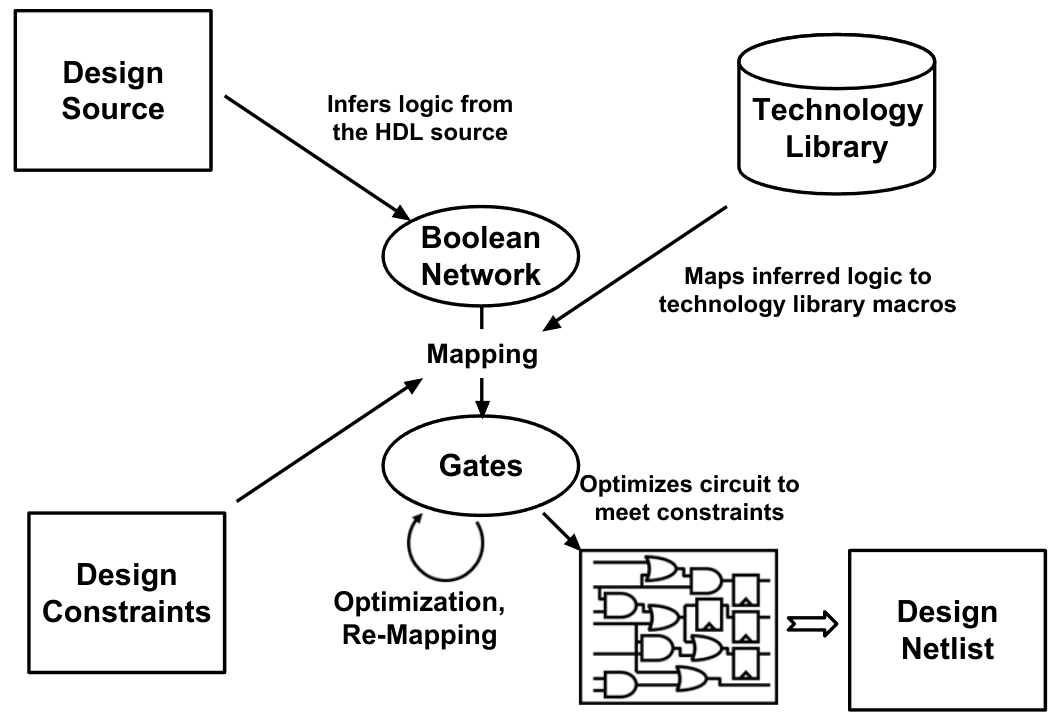
\includegraphics[width=0.95\textwidth]{img/12_what_synth.png}
\end{figure}
\end{frame}
\note{
\scriptsize{
This diagram is of course very simplified. Synthesis technology continues to evolve and this course does not intend to describe its particulars anyway. In a very general sense:
\begin{itemize}
\item The tool first transforms HDL input into an internal Boolean network of sequential storage elements and the logic "cone" expressions that feed them.
\item The tool then does some logic restructuring, such as prune logic that does not drive anything and does not share common sub-expressions. It also at this point makes a guess about operator implementation, basing its choice on expression length. For example, for a add operation it might choose a carry look-ahead added instead of a ripple-carry added based on operand width.
\item The tool next maps the design to the gates actually available in the target library and performs optimizations based on our constraints and the actual parameters of those gates.
\end{itemize}

}
}

%%%%%%%%%%%%%%%%%%%%%%%%%%%%%%%%%%%%%%%%%%%%%%%%%%%%%%%%%%%%
\begin{frame}
\frametitle{Synthesis in Our Design Flow}
\begin{figure}
    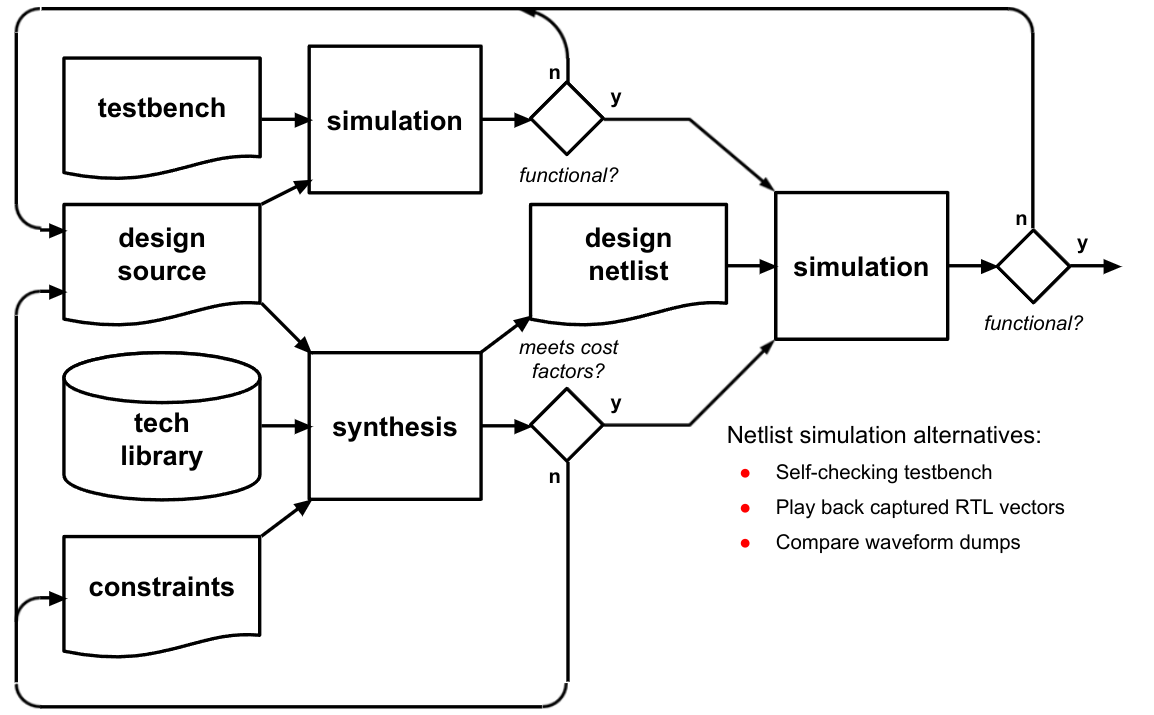
\includegraphics[width=0.95\textwidth]{img/12_flow_synth.png}
\end{figure}
\end{frame}
\note{
\tiny{
This high-level flow is applicable to all synthesis tools:
\begin{itemize}
\item The 1st major step is of course to develop the RTL design to the point where we are satisfied with its functionality. We should meanwhile be at least parsing the design blocks with the synthesis tool to ensure that it contains only acceptable RTL constructs and that the inferred registers and latches are only those we mean to infer.
\item The 2nd major step is to define the expected environment for the overall design: the design clocks, the input drive strength and arrival time with respect to the clock, and the output load and required arrival time with respect to the clock. These are the constraints applied to the top level of the design.
\item The 3rd major step is to determine and execute our synthesis strategy. Depending upon the platform resources available and the size and complexity of the design, we might synthesize the entire design together or we might synthesize smaller design pieces using a top-down strategy that propagates constraints down or a bottom-up strategy that develops higher-level constraints based upon the estimated timing of previously synthesized sub-designs. In any case, we record our strategy as commands in a script file that executes the synthesis strategy. Synthesis is an iterative process as we refine the strategy, constraints, and even the RTL, to meets the constraints of the operating environment.
\item The 4th major step, after the synthesized design meets the constraint of the operating environment, is to verify that the post-synthesis structural design is functionally equivalent to the pre-synthesis RTL design. Many teams accomplish this using the same test environment as for the RTL design. There are tools that can do this verification statically, as formal equivalence checking, and as time goes on, more teams choose to include such formal methods in their verification flow.
\end{itemize}

}
}

%%%%%%%%%%%%%%%%%%%%%%%%%%%%%%%%%%%%%%%%%%%%%%%%%%%%%%%%%%%%
\begin{frame}
\frametitle{Logic Inference Is Literal}
Synthesis tools infer logic from HDL structure and statements.
\begin{itemize}
\item They then optimize the logic as needed to meet constraints.
\item Here the $==$ operator is redundant but could still appear in the netlist.
\end{itemize}
\begin{figure}
    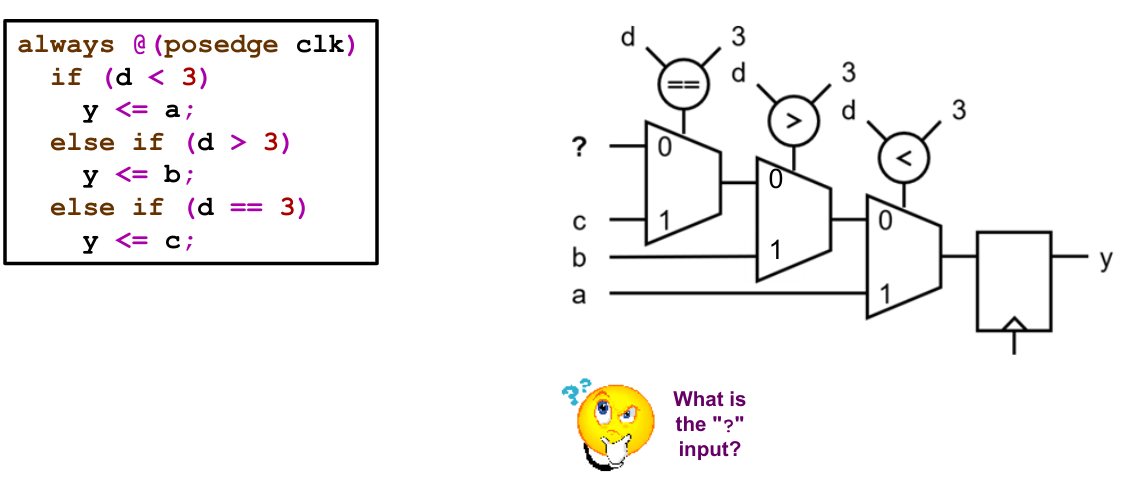
\includegraphics[width=0.95\textwidth]{img/12_inference.png}
\end{figure}
\end{frame}
\note{
\scriptsize{
Synthesis tools do not interpret or analyse our code to understand our intention. They initially transform our RTL design to Boolean logic quite literally, and then optimize it. They stop optimization when the design meets our requirements or they run out of time. For any non-trivial design, synthesis produces an optimization that is hopefully "good enough" but not likely to be perfect.
\newline

We can help the optimization process by explicitly organizing and coding our design as closely as possible to what we want the optimized result to look like. Write RTL but "think" hardware. A later module discusses such RTL coding \textit{best practices} for synthesis.

}
}

%%%%%%%%%%%%%%%%%%%%%%%%%%%%%%%%%%%%%%%%%%%%%%%%%%%%%%%%%%%%
\begin{frame}
\frametitle{Coding Style Affects Results}
Synthesis tools infer logic from HDL structure and statements.
\vspace{10pt}
\begin{itemize}
\footnotesize{
\item Logic synthesis tools do not insert storage elements.
\begin{itemize}
	\footnotesize{
	\item[$-$] Pipeline consideration (number of registers) are totally our responsibility.
	}
\end{itemize}
\item Some logic synthesis tools can move storage elements upstream or downstream in combinational logic to balance delays.
\item The quality of results depend mainly on code.
}
\end{itemize}
\end{frame}
\note{
\scriptsize{
A synthesis tool does not optimize the registers or latches in our design. We need to be careful how we structure our registered processes so that we only infer the registers we need. Check synthesis reports carefully to make sure.
\newline

We also need to be careful how much combinational logic is placed between adjacent register banks. If we place a 32-bit multiplier between adjacent register banks with a 10ns clock period, we shouldn't be surprised if the synthesis tool struggles to produce a result.
\newline

Generally, we need to be careful how we partition and structure our design and structure our design into combinational and registered logic.

}
}

%%%%%%%%%%%%%%%%%%%%%%%%%%%%%%%%%%%%%%%%%%%%%%%%%%%%%%%%%%%%
\begin{frame}
\frametitle{What Synthesis Sometimes Can't Do Well}
\begin{itemize}
\item Clock threes
\begin{itemize}
	\item[$-$] Usually require detailed, accurate net delay information
\end{itemize}
\item Complex clocking schemes
\begin{itemize}
	\item[$-$] Synthesis tools prefer simple, single clock synchronous designs
\end{itemize}
\item memory, IO pads, technology-specific cells
\begin{itemize}
	\item[$-$] We will probably need to instantiate these by hand
\end{itemize}
\item Synthesis tools can analyse hundreds of potential implementations in much less time than we need to analyse just one.
\end{itemize}
\end{frame}
\note{
\scriptsize{
Logic synthesis primarily targets for optimization of the logic cones between registers. Some things that require special handling are, for example:
\begin{itemize}
\item Clock tree design is a global, chip-wide problem which particularly in deep sub-micron designs requires detailed and realistic net delay information. No single clock tree generation method can apply to all designs. We will likely need to design the clock tree later as a part of silicon layout.
\item Synthesis tools typically have difficulty with complex clocking schemes. Synthesis works most reliably with a single clock per RTL module, and some tools restrict us to at most two clocks or require that the multiple clocks are harmonically related.
\item We may have to manually instantiate I/O cells and large regularly structured cells that synthesis tools do not readily select. We may want to utilize the technology vendor's silicon compilers to generate such large regularly-structured data-path elements and large memory blocks.
\end{itemize}
For any non-trivial design, synthesis produces an optimization that is hopefully good enough but not likely to be perfect. For a critical path that does not meet timing requirements, it is quite possible that we manually examine the path and find some way to improve it.

}
}

%%%%%%%%%%%%%%%%%%%%%%%%%%%%%%%%%%%%%%%%%%%%%%%%%%%%%%%%%%%%
\begin{frame}
\frametitle{Technology Specific Issues}
\begin{itemize}
\item Each technology suggests its own optimal architecture, with architecture-specific "tricks" for good utilization and speed.
\item Code becomes technology specific.
\item Refer to vendor literature.
\end{itemize}
\begin{figure}
    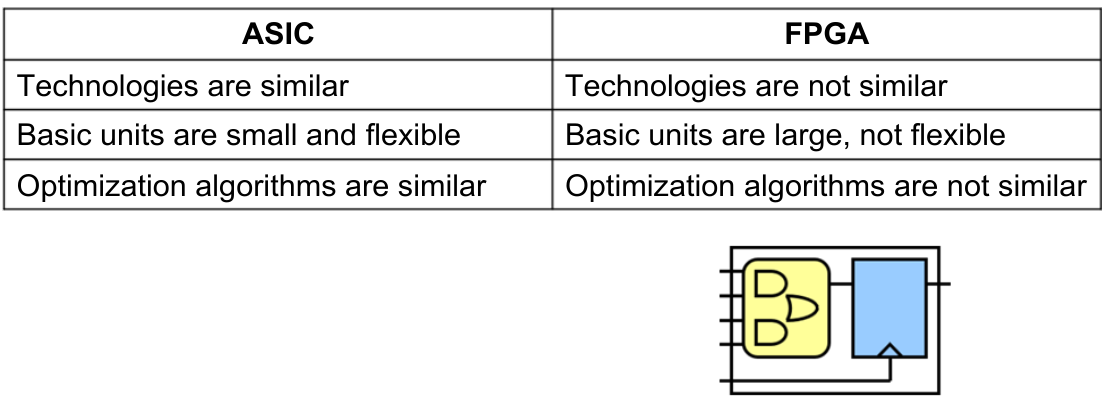
\includegraphics[width=0.95\textwidth]{img/12_tech_issues.png}
\end{figure}
\end{frame}
\note{
\scriptsize{
Each technology suggests its own optimal architecture, with architecture-specific "tricks" for good utilization and speed. To understand these differences, let's compare synthesis of an ASIC to synthesis of an FPGA:
\begin{itemize}
\item Synthesis of an ASIC is similar for all technologies - the library cells are relatively small and similar between technologies, routing delays are relatively more predictable, and the tools use basically the same optimization algorithms.
\item Synthesis of an FPGA can vary widely between technologies - the FPGA can by EEPROM, SRAM, or anti-fuse, each vendor has different building blocks that tend to be relatively large, and an FPGA architecture is relatively inflexible, leading to relatively widely-varying routing delays. FPGA design employs technology-specific and architecture-specific tricks, implemented as user-defined attributes, comments or direct instantiation, which are difficult for a synthesis tool to implement, thus making our Verilog code technology dependent and reducing its portability.
\end{itemize}

}
}

%%%%%%%%%%%%%%%%%%%%%%%%%%%%%%%%%%%%%%%%%%%%%%%%%%%%%%%%%%%%
\begin{frame}
\frametitle{Programmable Logic Device Specific Issues}
\scriptsize{
\begin{multicols}{2}
\begin{itemize}
\item Different architectures for different technologies
\item Fixed architecture within a specific technology
\item Architecture specific "tricks" for best utilization/speed
\item Technology specific/generic code trade-off
\item How our synthesis tools handles our technology
\end{itemize}
\vfill
\columnbreak
\begin{figure}
    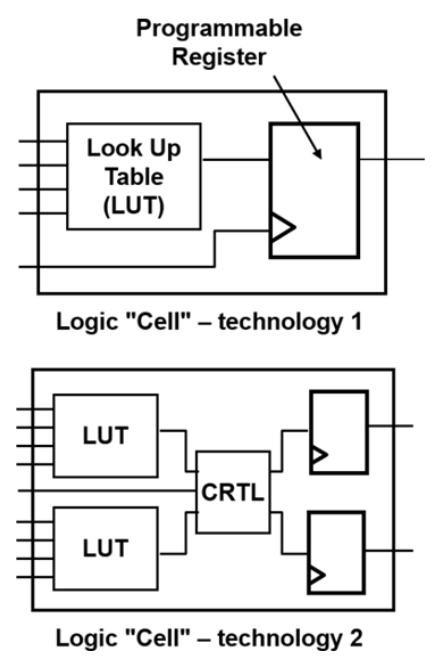
\includegraphics[width=0.35\textwidth]{img/12_programmable_issues.png}
\end{figure}
\end{multicols}
}
\end{frame}
\note{
\scriptsize{
Many of the comments so far have assumed synthesis to an ASIC. With an FPGA there are some different problems. ASIC synthesis tools all work in the same way, using the same optimization algorithms, and the target technology libraries all have similar cells. With FPGA there are different technologies, EEPROM, SRAM and anti-fuse, and each vendor has different building blocks, which tend to be much larger than the gate-level primitives used in an ASIC.
\newline

For a particular FPGA, the architecture is fixed, limiting the usefulness of static timing analysis since routing delays can vary widely - with an ASIC they are much more predictable. What's more, to get a good "fit" the FPGA designer traditionally employs architecture specific tricks which are difficult to implement in a synthesis tool.
\newline

HDL code may need to make use of the technology-specific techniques and tricks. These may be expresses with user-defined attributes, comments or direct instantiation of specific cells. Such techniques restrict the technology independence and portability of our code, but allows the most efficient implementation with a specific technology.
\newline

A key issues is how well our synthesis tool handles our chosen technology. To achieve a good result, it will need architecture specific algorithm.

}
}

%%%%%%%%%%%%%%%%%%%%%%%%%%%%%%%%%%%%%%%%%%%%%%%%%%%%%%%%%%%%
\begin{frame}
\frametitle{Synthesizable Verilog}
IEEE Std. 1364.1 defines the synthesizable Verilog constructs.
\scriptsize{
\begin{multicols}{2}
\begin{itemize}
\item Not all synthesis tools yet accept all the standard constructs.
\end{itemize}
\vfill
\columnbreak
\begin{itemize}
\item Most synthesis tools still accept also their own legacy constructs.
\end{itemize}
\end{multicols}
}
\begin{figure}
    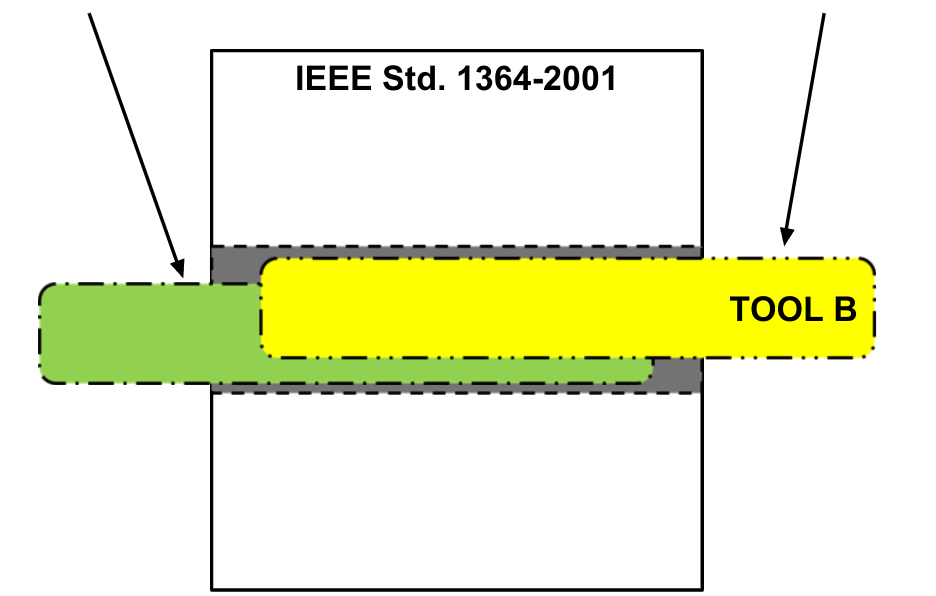
\includegraphics[width=0.75\textwidth]{img/12_synthesizable.png}
\end{figure}
\end{frame}
\note{
\scriptsize{
The IEEE Std. 1364.1-202 for Verilog RTL synthesis describes use of the Verilog "synthesizable subset" in a manner from which logic synthesis tools can infer logic.
\begin{itemize}
\item We will rarely but perhaps occasionally use a logic synthesis tool that does not accept some standard synthesizable constructs.
\item As logic synthesis existed long before the standard, the predominant tools still support construct that did not become standard.
\item This course describes what is standard. If we write our RTL code according to this cource, then our code will be portable between the maximum number of synthesis tools.
\end{itemize}

}
}

%%%%%%%%%%%%%%%%%%%%%%%%%%%%%%%%%%%%%%%%%%%%%%%%%%%%%%%%%%%%
\begin{frame}
\frametitle{Module Summary}
We should now be able to briefly describe what is synthesis.
\newline

This module described:
\begin{itemize}
\item What we provide to the synthesis tool:
\begin{itemize}
	\scriptsize{
	\item[$-$] Design source, design constraints, technology library
	}
\end{itemize}
\item What the synthesis tool does:
\begin{itemize}
	\scriptsize{
	\item[$-$] infers logic from the HDL source, maps the inferred logic to technology library macros, and optimizes the circuit to meed constraints
	}
\end{itemize}
\item What the synthesis tool might need help with:
\begin{itemize}
	\scriptsize{
	\item[$-$] Complex clocking schemes, large memories, I/O pads 
	}
\end{itemize}
\item What part of Verilog is synthesizable:
\begin{itemize}
	\scriptsize{
	\item[$-$] Defined by the IEEE Std. 1364.1 
	}
\end{itemize}
\end{itemize}
\end{frame}
\note{
\scriptsize{
This module explored the basics of synthesis - how it works, where it fits in our flow, its strengths and weaknesses, and some things to watch for.

}
}

%%%%%%%%%%%%%%%%%%%%%%%%%%%%%%%%%%%%%%%%%%%%%%%%%%%%%%%%%%%%
\begin{frame}
\frametitle{Module Review}
\scriptsize{
\begin{enumerate}
\item What are the user-provided inputs to logic synthesis?
\item \textbf{True or False?} Given multiple different functionally accurate descriptions of a design function, a synthesis tool will for each produce the exact same one "best" implementation.
\item What design blocks might we need to instantiate rather then infer?
\item What entity determines how we must code Verilog designs for inference by a logic synthesis tool?
\end{enumerate}
}
\end{frame}
\note{
\scriptsize{
\begin{enumerate}
\item What are the user-provided inputs to logic synthesis?
\begin{itemize}
	\tiny{
	\item The logic synthesis user must provide the design source, design constraints, and target technology library.
	}
\end{itemize}
\item \textbf{True or False?} Given multiple different functionally accurate descriptions of a design function, a synthesis tool will for each produce the exact same one "best" implementation.
\begin{itemize}
	\tiny{
	\item False. A synthesis tool infers logic exactly as described, and then optimizes it to meed constraints. It stops when it meed constraints or exceeds the computational limits we set.
	}
\end{itemize}
\item What design blocks might we need to instantiate rather then infer?
\begin{itemize}
	\tiny{
	\item We are likely to instantiate rather than infer large memories and I/O pads, and potentially at least partially instantiate clock trees.
	}
\end{itemize}
\item What entity determines how we must code Verilog designs for inference by a logic synthesis tool?
\begin{itemize}
	\tiny{
	\item The "IEEE Standard for Verilog Register Transfer Level Synthesis" determines how we must code Verilog designs for inference by a logic synthesis tool.
	}
\end{itemize}
\end{enumerate}

}
}

%%%%%%%%%%%%%%%%%%%%%%%%%%%%%%%%%%%%%%%%%%%%%%%%%%%%%%%%%%%%
\begin{frame}
\frametitle{Lab}
Lab 13-1: Exploring the Synthesis Process
\begin{itemize}
\item For this lab, we will synthesize a small multiplexor model and examine the results.
\end{itemize}
\end{frame}



%%%%%%%%%%%%%%%%%%%%%%%%%%%%%%%%%%%%%%%%%%%%%%%%%%%%%%%%%%%%
\begin{frame}
\frametitle{Test You Understanding - 1}
Which one or more of these do you provide to a logic synthesis tool?
\begin{itemize}
\item[$\square$] Number of pipeline stages
\item[$\square$] Technology library
\item[$\square$] Timing constraints
\item[$\square$] Design source
\end{itemize}
\end{frame}
\note{
Which one or more of these do you provide to a logic synthesis tool?
\begin{itemize}
\item[$\square$] Number of pipeline stages
\item[$\boxtimes$] Technology library
\item[$\boxtimes$] Timing constraints
\item[$\boxtimes$] Design source
\end{itemize}
}

%%%%%%%%%%%%%%%%%%%%%%%%%%%%%%%%%%%%%%%%%%%%%%%%%%%%%%%%%%%%
\begin{frame}
\frametitle{Test You Understanding - 2}
Who determines how you must code Verilog designs for inference by a logic synthesis?
\begin{itemize}
\item[$\square$] Accelera
\item[$\square$] Cadence Design Systems
\item[$\square$] Institute for Electrical and Electronics Engineers (IEEE)
\item[$\square$] Synopsys
\end{itemize}
\end{frame}
\note{
Who determines how you must code Verilog designs for inference by a logic synthesis?
\begin{itemize}
\item[$\square$] Accelera
\item[$\square$] Cadence Design Systems
\item[$\boxtimes$] Institute for Electrical and Electronics Engineers (IEEE)
\item[$\square$] Synopsys
\end{itemize}
}

\end{document}
